\chapter{Metodología e implementación}
Con la idea de facilitar el trabajo y eliminar errores a la hora de realizar los cálculos, se desarrolló una aplicación visual que permite a un usuario introducir la cronología de huracanes, el programa le brindara una serie de opciones desarrolladas para filtrar los datos en distintas cronologías de huracanes ya sea a nivel de país (Cuba), por región o por provincia; y apreciar distintos análisis de los mismos para definir los períodos de retorno de huracanes a través del modelo de Poisson con el objetivo de agilizar y obtener rápidamente información. 
La herramienta computacional que se presenta en este documento es una aplicación de nombre \textbf{TkHURSv1.1}, desarrollada sobre la plataforma \textit{.NET} y utilizando el lenguaje de programación C\#. En este capítulo presentaremos la metodología utilizada en el software para analizar el comportamiento de los huracanes. 
%Esta investigación fue parte del diploma de un estudiante de Ciencia de la Computación de la facultad de Matemática y Computación de la Universidad de la Habana.

\section{Entorno de desarrollo}
A continuación se describen las plataformas y herramientas escogidas para el desarrollo de la aplicación. 

\subsection{Plataforma .NET}

La plataforma  \textit{.NET}, en inglés \textit{.NET Framework}, fue desarrollada por \textit{Microsoft} con el objetivo de obtener una plataforma sencilla y potente que funcionara sobre \textit{Windows} e integrara un número de tecnologías surgidas durante el fin de la década de 1990. Esta plataforma consta de cuatro grupos de componentes \cite{DK2}:

\begin{itemize}
\item  Herramientas de desarrollo y bibliotecas: Es un conjunto conformado por lenguajes de programación (entre ellos C\#, Visual Basic.Net y F\#), herramientas de desarrollo como Visual Studio, una biblioteca de clases integral para construir aplicaciones tanto para la web como para \textit{Windows}.

\item Servicios Web: Oferta de servicios web comerciales, por una cuota los desarrolladores pueden usarlos para desarrollar aplicaciones que los requieran.

\item Servidores especializados: Son un grupo de servidores empresariales, entre ellos se encuentra el SQL Server.

\item Dispositivos: Es la posibilidad de interactuar con dispositivos que no sean computadoras, como teléfonos celulares o dispositivos de juego.
\end{itemize}


Cuando las aplicaciones desarrolladas sobre \textit{.NET} son compiladas, se genera un código intermedio entre el lenguaje de programación utilizado y el código de máquina. A este código intermedio se le conoce como \textit{Common Intermediate Language (CIL)}. Cuando una aplicación es ejecutada, la plataforma \textit{.NET} se encarga de convertir el código \textit{CIL} en código de máquina. Este proceso se basa en dos pilares fundamentales \cite{DK2, DK8}:  

\begin{itemize}
\item  Common Language Runtime (CLR): Es el entorno de ejecución que pasa de código intermedio CIL a código máquina y permite ejecutar cualquier aplicación en cualquier entorno.

\item Framework Class Library (FCL): Son las bibliotecas de clase, incluidas en la plataforma, que permiten acceder a los servicios ofrecidos por el CLR y las funcionalidades más usadas a la hora de escribir programas.
\end{itemize}

Existen varias versiones de la plataforma \textit{.NET}, la primera de ella fue lanzada en el año 2002 y fue conocida como \textit{.NET Framework 1.0}. Ha seguido continuamente su desarrollo, hasta la última versión, \textit{.NET Framework 4.8}, lanzada el 18 de Abril de 2019\cite{DK8}. En cada nueva versión de la plataforma, se incluyen nuevas funcionalidades, servicios y mejoras en los lenguajes de programación. La aplicación \textbf{TkHURSv1.1}, propuesta en este trabajo fue desarrollada sobre la plataforma \textit{.NET Framework 4.5}, aunque es más acertado decir que se siguió desarrollando en dicha plataforma porque este proyecto es una actualización de una versión anterior. Pero la plataforma utilizada es capaz de proveer los recursos necesarios para la tarea en cuestión.%por ser mucho más distribuida que la reciente versión 4.6 y por el gran número de bibliotecas de clases compatibles.

\subsection{Lenguaje de programación C\#}

El nombre C\# viene del inglés “C Sharp”. C\# fue en su día el nuevo lenguaje diseñado por Microsoft para su plataforma \textit{.NET}. Sus principales creadores fueron Scott Wiltamuth y Anders Hejlsberg, éste último también conocido por haber sido el diseñador del lenguaje Turbo Pascal y la herramienta RAD Delphi.
C\# es un lenguaje de programación que toma las mejores características de lenguajes preexistentes como Visual Basic, Java y C++ y las combina en uno solo. El hecho de ser relativamente reciente no implica que sea inmaduro, pues \textit{Microsoft} ha escrito la mayor parte del FCL usándolo, por lo que su compilador es el más depurado y optimizado de los incluidos en el \textit{.NET Framework} \cite{DK0, DK9}.

Por características de este lenguaje como son la sencillez, orientación a objetos y gestión automática de memoria, se escogió para el desarrollo de la aplicación propuesta. A continuación se describen estas características: 

\begin{itemize}
\item Sencillez: Elimina muchos elementos que otros lenguajes incluyen y que son innecesarios en \textit{.NET}.

\item Orientación a Objetos: Como todo lenguaje de programación de propósito general actual, C\# es un lenguaje orientado a objetos. La diferencia de este enfoque orientado a objetos respecto al de otros lenguajes como C++ es que el de C\# es más puro en tanto que no admiten ni funciones ni variables globales sino que todo el código y datos han de definirse dentro de definiciones de tipos de datos, lo que reduce problemas por conflictos de nombres y facilita la legibilidad del código.

\item Gestión automática de memoria: Todo lenguaje de \textit{.NET} tiene a su disposición el recolector de basura del CLR, el cual libera automáticamente las zonas de memoria que no son utilizadas. Esto tiene el efecto en el lenguaje de que no es necesario incluir instrucciones de destrucción de objetos.
\end{itemize}

\section{Funcionalidades del software}

El software \textbf{TkHURSv1.1} ofrece una gama de opciones para el trabajo con cronologías de huracanes. Su funcionamiento comienza con la importación de datos de un fichero csv con el siguiente formato: la primera columna debe tener los nombres de los huracanes o como fueron conocidos, la segunda el año de la afectación, la tercera el mes en que afectaron y la cuarta los días, el resto de las columnas representan como afectó a cada una de las provincias en la escala Saffir-Simpson representado por un número de 1 al 5.\\


Los encabezados de las columnas de las provincias deben coincidir con los especificados en la ventana “Leyenda” de la aplicación para cada una de las mismas. Una vez cargados estos datos, se permitirán seleccionar distintas opciones para visualizar los datos y facilitar el trabajo del especialista del Instituto de Meteorología. Se podrá observar la cronología cargada, así como, editar las entradas existentes y agregar nuevas. Se podrán cargar nuevas cronologías\footnote{La aplicación solo trabaja con una cronología a la vez.} y, para facilitar el trabajo del investigador, recuerda la última cronología usada y la importa automáticamente al ejecutar la aplicación.\\


La nueva versión del software está pensada para que sea intuitiva y de fácil manejo para los usuarios a los que está destinado, así como su predecesor. Se proporcionan una serie de filtros para optimizar la vista de los datos deseados. Entre los parámetros que permiten ser modificados para el funcionamiento de los filtros se encuentran: rango anual, rango de categoría y región o provincia que se desea observar.
Se muestra el período de tiempo observado y la cantidad de huracanes en cada vista. Entre las distintas pantallas que se ven afectadas por el filtrado se encuentran: una vista simple de la cronología restringida, cantidad de huracanes por categoría, cantidad de huracanes coincidentes en el mismo año por categoría, cantidad de huracanes por meses, los gráficos de barras, pastel y línea, algunos de los cuales tienen sus propias opciones para personalizar la forma en la que se quiere observar los datos deseados, también el mapa (en desarrollo) se incluye en esta lista; y una tabla mostrando el período de retorno de los huracanes, con distintas frecuencias de la estadística descriptiva y varios cálculos para facilitar la aplicación de la comprobación de $\chi^{2}$ y Kolmogorov-Smirnov, todo esto explicado en la sección 1.1.\\

Además, se proporciona una leyenda para el conocimiento del usuario de todas las variables y abreviaturas usadas y sus respectivos significados (Figura \ref{fig:Leyenda}). Se permite, también, la exportación de todas las tablas obtenidas a un archivo .xls de Microsoft Excel. La Figura \ref{fig:esquema_metodologia} muestra, en un simple esquema, el flujo de la aplicación.\\

\section{Metodología}

En esta sección se exponen los pasos básicos para el uso de esta aplicación de escritorio:
\begin{description}

\item[PASO 1:]{ En Archivo, Cargar Cronología: se cargan los datos desde un fichero .csv.}

\item[PASO 2:]{ En Mostrar, Cronología General: se muestra la tabla de toda la información.}

\item[PASO 3:]{ En Años: se define el año de inicio y final.} 

\item[PASO 4:]{ En Categoría: se elige una o varias categorías de los huracanes.}

\item[PASO 5:]{ En Región: se elige la provincia, la región o Cuba en general.}

\item[PASO 6:]{ Escoger el modo de obsevar la información en menú “Visualización”. Hay 3 opciones principales: Modo Tabla (mostrada por defecto en caso de que no se escoja ninguna en principio), Modo Gráfico (el cual trae 3 opciones más: Gráfico de Barras, Gráfico de Pastel y Gráfico de Línea) y Modo Mapa.}

\item[PASO 7:]{ Una vez realizados los pasos 3, 4, 5 y 6, se muestra la información con la visualidad escogida por el usuario automáticamente. Cabe aclarar que, a excepción de la vista ``Cronología General'', todas las demás son afectadas por los filtros aplicados: el resto de tablas y todos los gráficos.}


\begin{itemize}

\item En Mostrar, Huracanes/Categoría: se muestra la tabla del conteo de Huracanes por Categorías en la escala de Saffir-Simpson.

\item En Mostrar, Huracanes al Año/Categoría: se muestra la tabla del conteo de cuántas veces han ocurrido cierta cantidad de huracanes al año de cada una de las categorías según la escala de Saffir-Simpson.

\item En Mostrar, Períodos de Retorno: se muestran varias informaciones de interés como la frecuencia observada y esperada del número de huracanes, y lo más importante los valores del período de retorno de cada cantidad específica de huracanes por año. Se muestra el cálculo de la prueba de $\chi^{2}$ y Kolmogorov-Smirnov. En esta versión es posible escoger parte de la información a mostrar en dicha tabla (Figura \ref{fig:Periodos_retorno}).

\item En Mostrar, Meses/Categorías: se puede observar el conteo de los huracanes por mes y categoría. Muestra la cantidad de huracanes de los tres meses más activos (agosto, septiembre y octubre) y la cantidad de huracanes intensos (categorías 3, 4 y 5 en la escala de Saffir-Simpson).

\item En Guardar Cambios: se puede guardar cualquier cambio que se realice en la misma vista de la aplicación, creando un nuevo fichero que se puede guardar con el nombre deseado.

\item En Leyenda: esta pestaña se encarga, solamente, de proporcionar una leyenda sobre la simbología usada en la aplicación en general para una mayor comprensión.

\item En la pantalla se pueden observar la cantidad de huracanes y el período de tiempo que se va a usar en el estudio deseado.

\end{itemize}

\item[PASO 8:]{ En Archivo, Guardar: se guarda en un fichero .xls los datos con los cuales se han realizado el análisis (Cronología General, Cronología Filtrada, Huracanes/Categoría, Huracanes Al Año/Categoría, Períodos de Retorno y Meses/Categoría) o se salva el gráfico observado en una imagen; dependiendo de que se muestre en la pantalla principal.}


\end{description}


Como resumen se ilustra gráficamente (Figura \ref{fig:esquema_metodologia}) la metodología utilizada en el software \textbf{TkHURSv1.1}.

\begin{figure}[H]
\centering
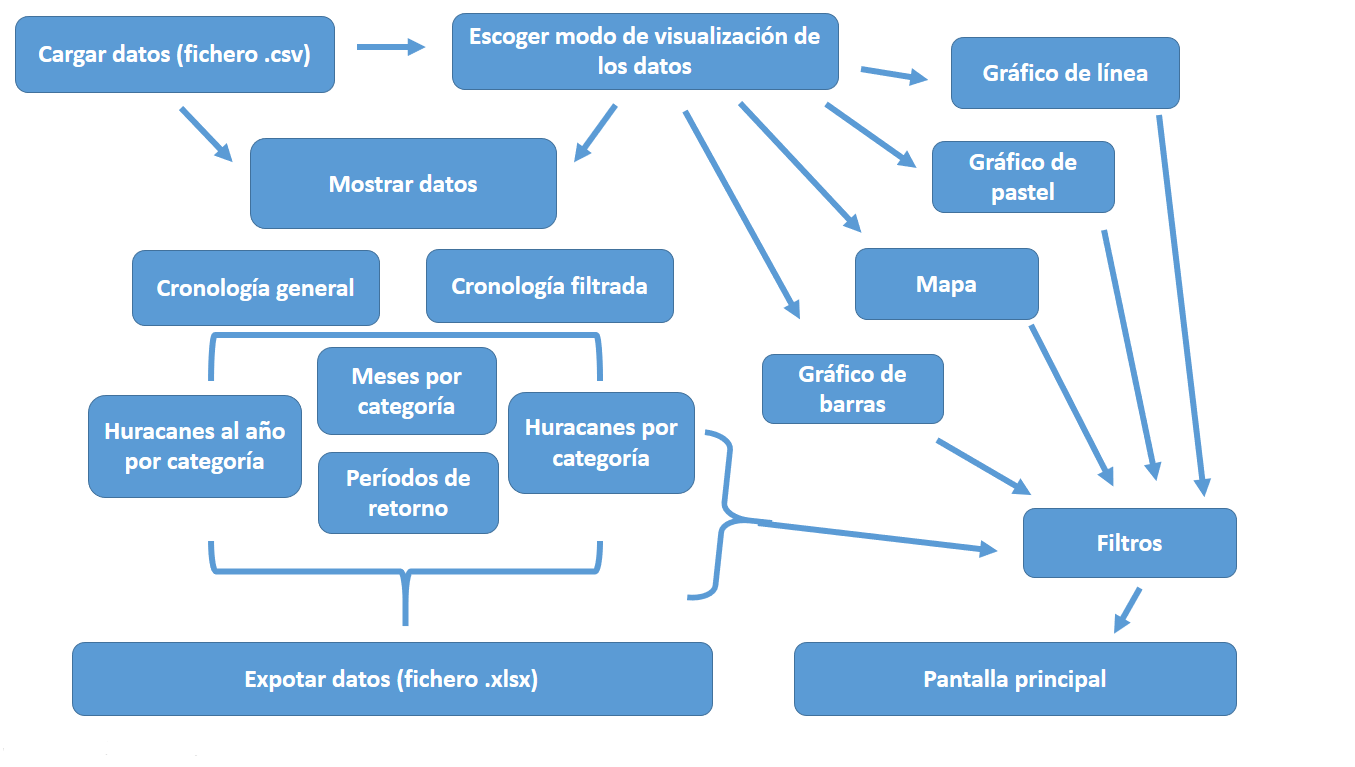
\includegraphics[scale=0.45]{esquema_metodologia}
\caption{Metodología seguida en el software TkHURSv1.1}
\label{fig:esquema_metodologia}
\end{figure}

\pagebreak

\section{Descripción del software}

\textbf{ TkHURSv1.1} es un software pensado para trabajar en él de forma intuitiva. Inclusive no cuenta con muchos comandos o botones para realizar la acción deseada con el objetivo de hacer su manejo lo más sencillo posible para el usuario. Es posible visualizar los datos en forma de tabla y gráfico lo que hace mucho más fácil las comparaciones o cualquier otro tipo de consulta que se quiera hacer con los datos proporcionados en el archivo ``.csv'' que se debió cargar previamente. 


\subsection{Pantalla principal}

Se brinda una breve descripción de las características del software que a nuestro entender son de gran importancia. La aplicación cuenta con una vista principal (Figura \ref{fig:Pantalla_principal_vacia}) compuesta por distintos componentes:
\\

\begin{figure}[H]
\centering
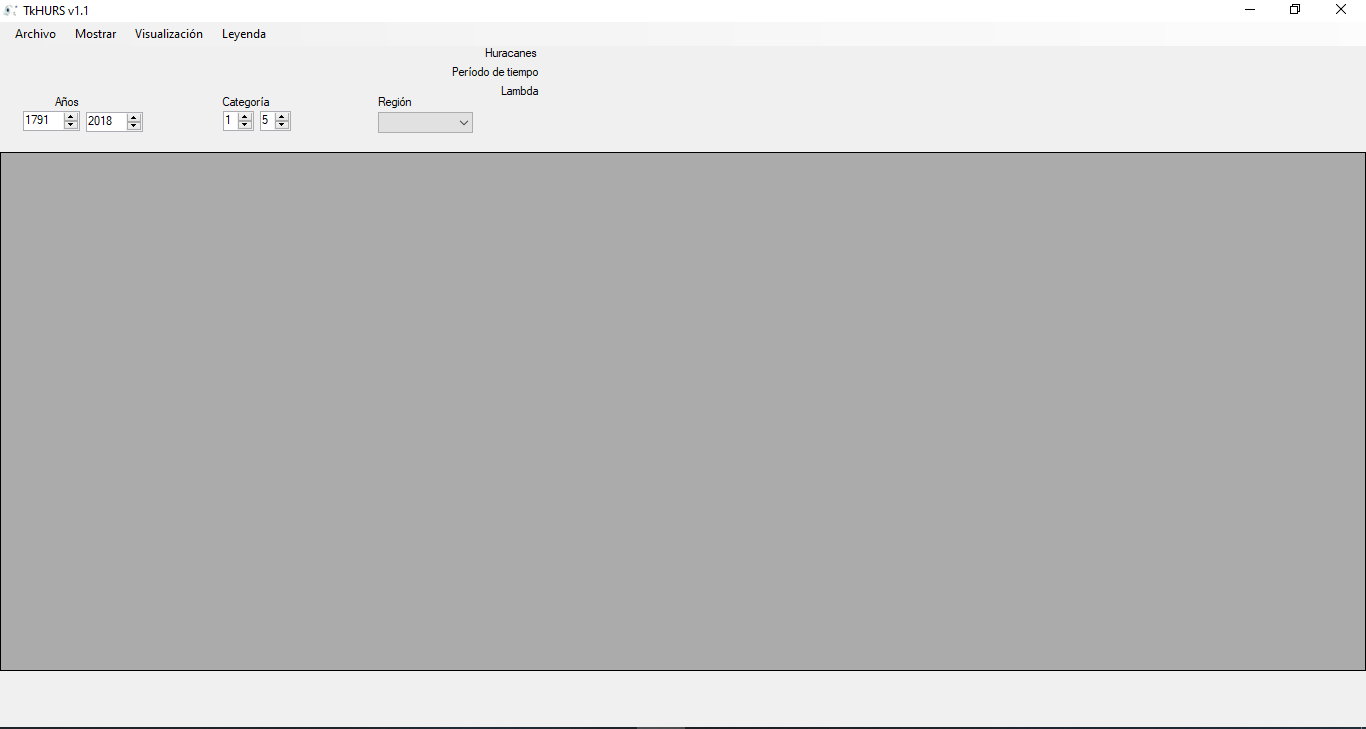
\includegraphics[scale=0.35]{Pantalla_principal_vacia}
\caption{Pantalla principal}
\label{fig:Pantalla_principal_vacia}
\end{figure}

\pagebreak

\begin{description}
\item[Archivo: ]{se usa para dos funciones: Cargar Cronología y Guardar.}

\item [Mostrar:] {se usa para seis funciones: Cronología General, Cronología Filtrada, Huracanes/Categoría, Huracanes Al Año/Categoría, Períodos de Retorno y Meses/Categoría.}

\item[Leyenda:] { esta pestaña se encarga de proporcionar la simbología usada en la aplicación.}

\item[Años:] permite elegir año de inicio y final para realizar distintos análisis sobre los datos.

\item[Categoría:]{ permite elegir una o varias categorías de los huracanes que se muestran.}

\item[Región:]{ permite elegir la provincia, la región o Cuba en general para realizar el análisis deseado.}

\item[Huracanes:]{ muestra la cantidad de huracanes.}

\item[Período de tiempo:]{ muestra la cantidad de años analizados.}

\item[Lambda:]{ muestra el valor estimado del parámetro poblacional lambda.}
\end{description}

\pagebreak

La imagen siguiente (Figura \ref{fig:Cronologia_general}) es otro de los estados de la aplicación: cuando se muestra la Cronología General surge otro elemento, el botón Guardar Cambios

\begin{figure}[H]
\centering
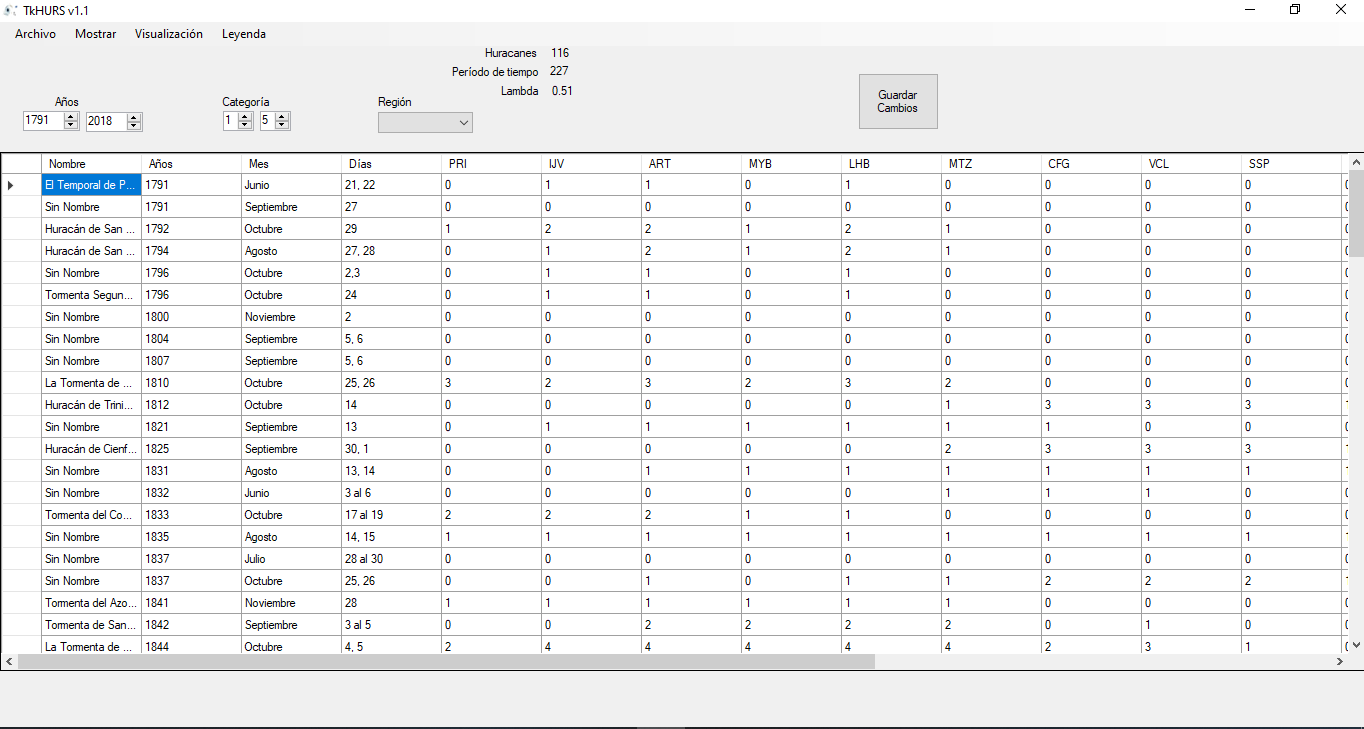
\includegraphics[scale=0.45]{Cronologia_general}
\caption{Pantalla principal con la cronología general cargada}
\label{fig:Cronologia_general}
\end{figure}


\begin{description}
\item[Guardar Cambios:]{ se usa para guardar cualquier cambio que se realice, creando un nuevo fichero que puede guardarse con el nombre deseado, sin afectar la cronología general.}
\end{description}

\pagebreak

\subsection{Entrada de los datos y descripción del fichero}

Parte principal del software es conocer los datos sobre los que se realizara el estudio. Para facilitarles a los usuarios la entrada de los mismos al programa se les brinda la opción de cargar un fichero ``.csv'' con la cronología, la cual se puede modificar y actualizar cada vez que sea necesario (Figura \ref{fig:Archivo_opciones}).


\begin{figure}[H]
\centering
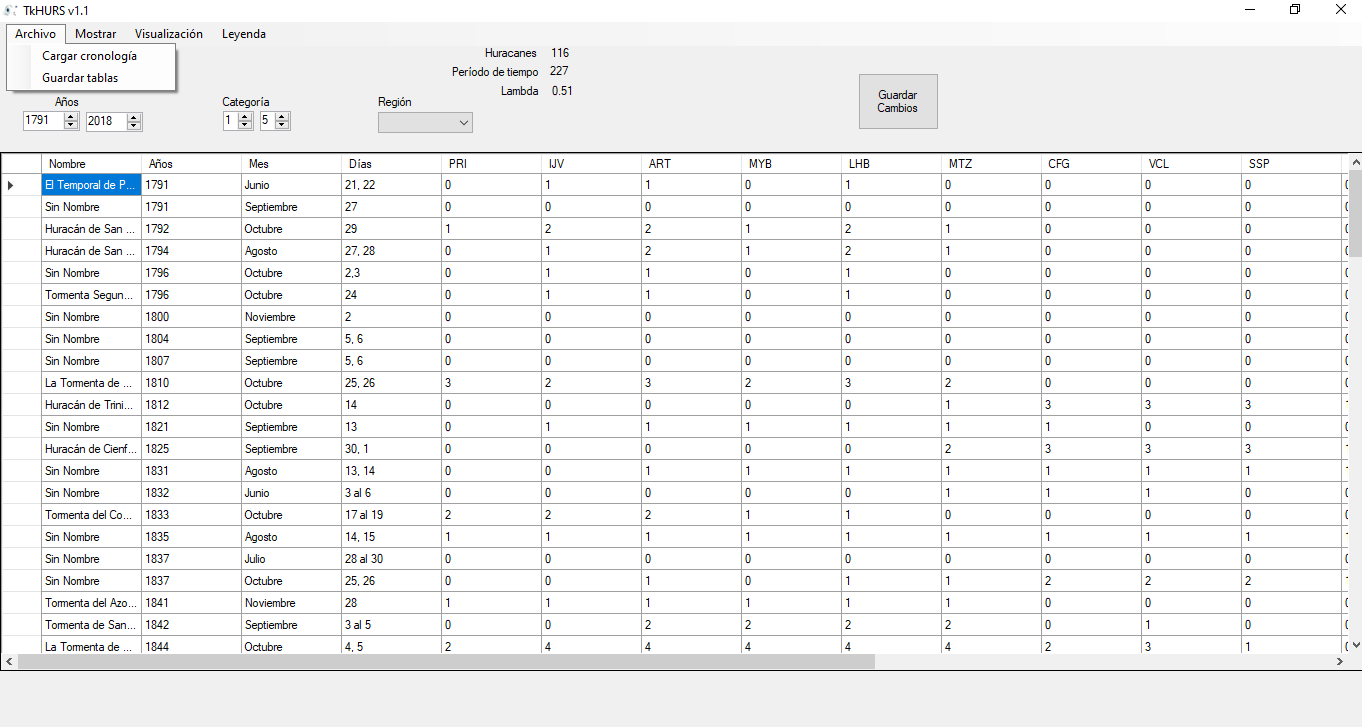
\includegraphics[scale=0.45]{Archivo_opciones}
\caption{Entrada de datos al sistema}
\label{fig:Archivo_opciones}
\end{figure}

\pagebreak

El fichero se describe de la siguiente manera: la primera columnas será el nombre del huracán, la segunda el año, la tercera el mes, la cuarta el o los días en que afectó al país y el resto de las columnas representarán con qué categoría afectó a cada una de las provincias. En caso de haber cargado los datos y querer seguir trabajando sobre ellos no es necesario volverla a cargar ya que la aplicación recuerda la última información cargada  (Figura \ref{fig:Fragmento_cronologia}).


\begin{figure}[H]
\centering
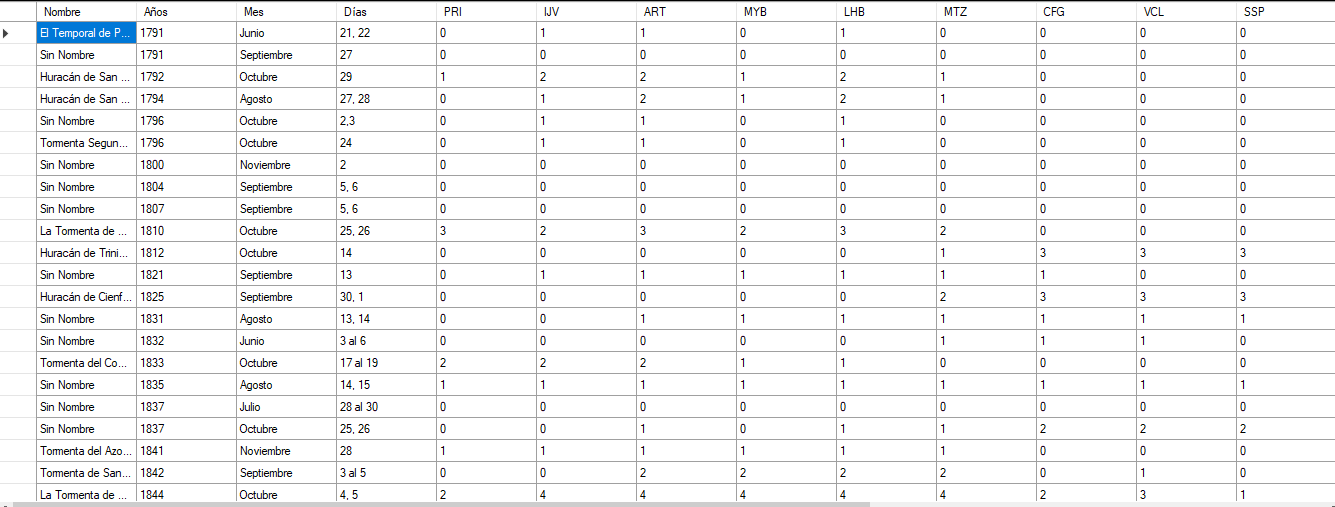
\includegraphics[scale=0.45]{Fragmento_cronologia}
\caption{Fragmento de la Cronología de huracanes de Cuba 1791-2018}
\label{fig:Fragmento_cronologia}
\end{figure}

\pagebreak

\subsection{Mostrar las distintas tablas y gráficos}

Con la opción ``Mostrar'' se pueden ver las distintas tablas acerca de los datos: Cronología General, Cronología Filtrada,Huracanes/Categoría, Huracanes Al Año/Categoría, Períodos de Retorno y Meses/Categoría (Figura \ref{fig:Mostrar_opciones}).\\

\begin{figure}[H]
\centering
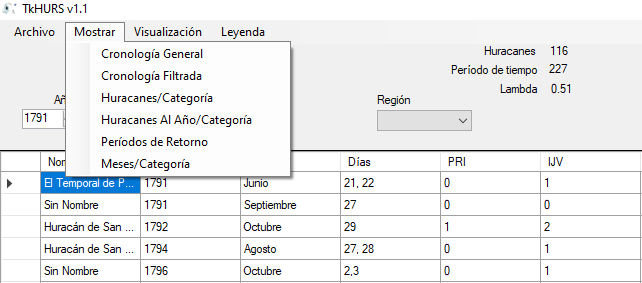
\includegraphics[scale=1]{Mostrar_opciones}
\caption{Se muestran las diferentes opciones de tabla}
\label{fig:Mostrar_opciones}
\end{figure}

Cada una de las vistas mencionadas con anterioridad van a ser explicadas con más detalle en breve para que se tenga una mejor idea del funcionamiento del software en cuestión \textbf{TkHURSv1.1}. Se espera que no haya dudas o al menos que se vean disminuidas después de esto.

\pagebreak

Cronología General: muestra la cronología cargada en su totalidad sin tener en cuenta filtros de ningún tipo (Figura \ref{fig:Cronologia_general1}). En esta vista es donde se pueden modificar y guardar los datos que se proveen en el archivo ``.csv''. Aquí es donde único se va a mostrar el botón ``Guardar Cambios'' que hace posible salvar las modificaciones realizadas.\\

\begin{figure}[H]
\centering
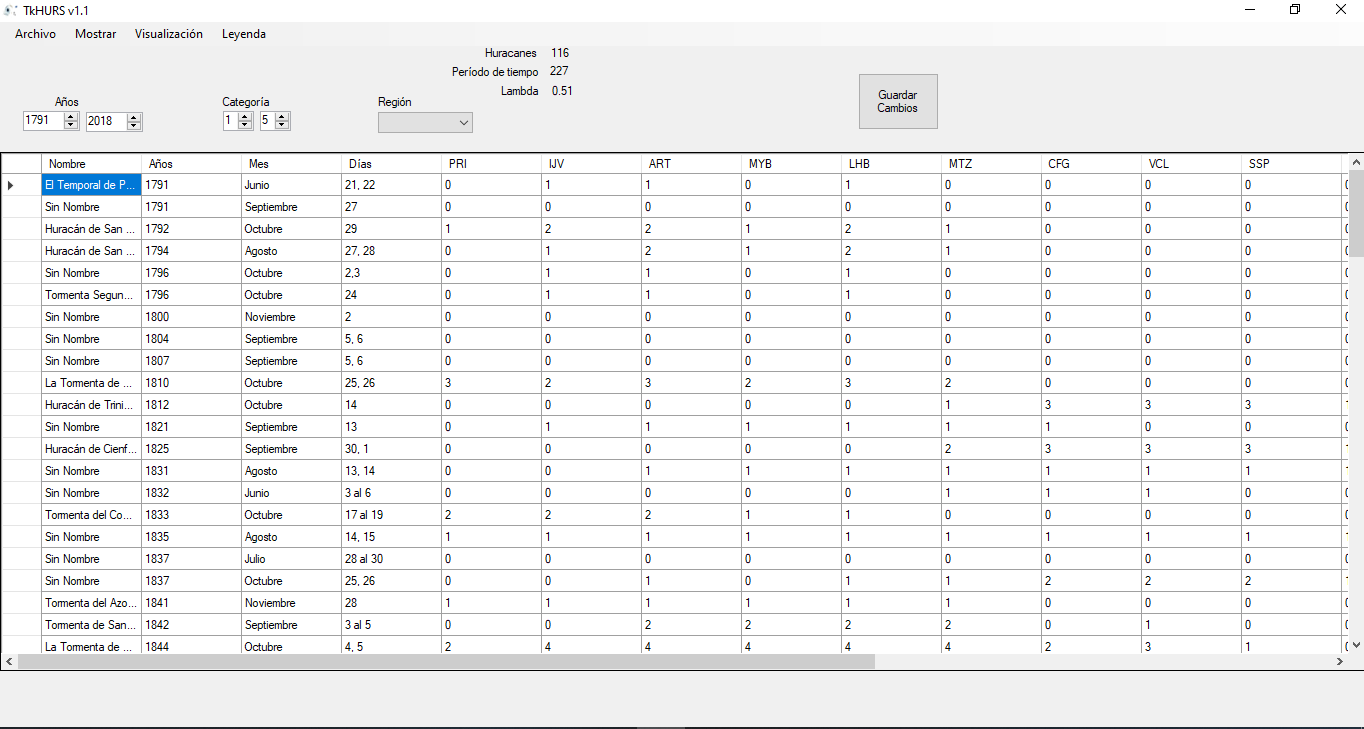
\includegraphics[scale=0.45]{Cronologia_general1}
\caption{Pantalla principal con la cronología general cargada}
\label{fig:Cronologia_general1}
\end{figure}

\pagebreak

Cronología Filtrada: muestra la cronología resultante de aplicar la selección de los datos del rango de años, de categoría y la región que se quiere investigar (Figura \ref{fig:Cronologia_filtrada}). Cabe destacar que a excepción de la opción ``Cronología general'', todas las opciones que siguen en lo adelante se ven afectadas por el filtro de la aplicación: el resto de las tablas, todos los gráficos y el mapa.\\


\begin{figure}[H]
\centering
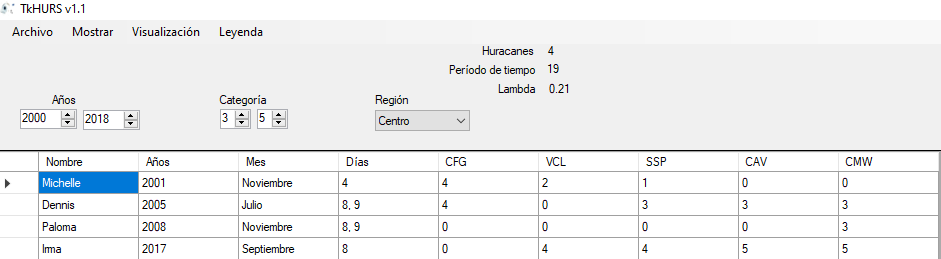
\includegraphics[scale=0.65]{Cronologia_filtrada}
\caption{Cronología filtrada}
\label{fig:Cronologia_filtrada}
\end{figure}

Huracanes/Categoría: muestra un conteo de los huracanes por categoría en la escala de Saffir-Simpson (Figura \ref{fig:Huracanes_categoria}).

\begin{figure}[H]
\centering
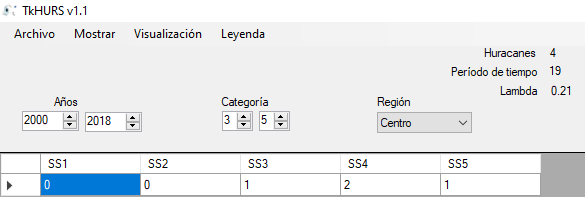
\includegraphics[scale=1]{Huracanes_categoria}
\caption{Huracanes por categorías}
\label{fig:Huracanes_categoria}
\end{figure}

\pagebreak


Huracanes al Año/Categoría: muestra un conteo de cuántas veces ha ocurrido cierta cantidad de huracanes al año de cada una de las categorías según la escala de Saffir-Simpson (Figura \ref{fig:Huracanes_ano_categoria}).

\begin{figure}[H]
\centering
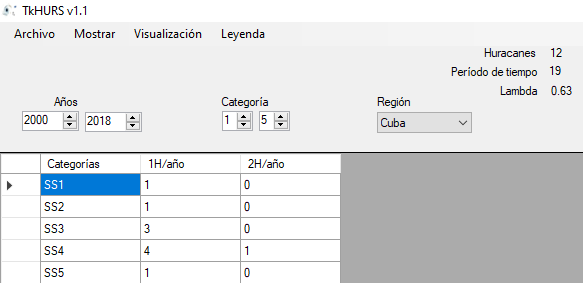
\includegraphics[scale=0.5]{Huracanes_ano_categoria}
\caption{Huracanes al año por categorías}
\label{fig:Huracanes_ano_categoria}
\end{figure}


Períodos de Retorno: esta es la función más importante de la aplicación porque aquí es donde se muestran los resultados calculados para el período de retorno de los huracanes para nuestro país; razón fundamental por la cual se decidió desarrollar esta aplicación de escritorio y por tanto parte vital en ella (Figura \ref{fig:Periodos_retorno}).

\begin{figure}[H]
\centering
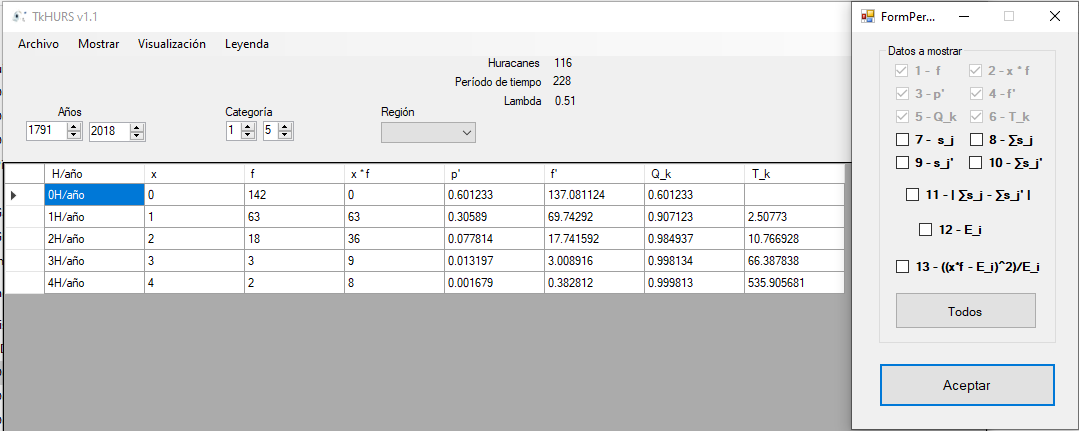
\includegraphics[scale=0.6]{Periodos_retorno}
\caption{Períodos de retorno}
\label{fig:Periodos_retorno}
\end{figure}

\pagebreak

Meses/Categoría: muestra un conteo de los huracanes por mes y categoría en la escala de Saffir-Simpson. Muestra en la última columna la cantidad de huracanes de los tres meses más activos (agosto, septiembre y octubre), sólo presenta ese valor; y la cantidad de huracanes intensos (categorías 3, 4 y 5 en la escala de Saffir-Simpson), valor observable en la última fila y solamente se ve ese resultado al igual que con los meses más activos (Figura \ref{fig:Meses_categoria}).

\begin{figure}[H]
\centering
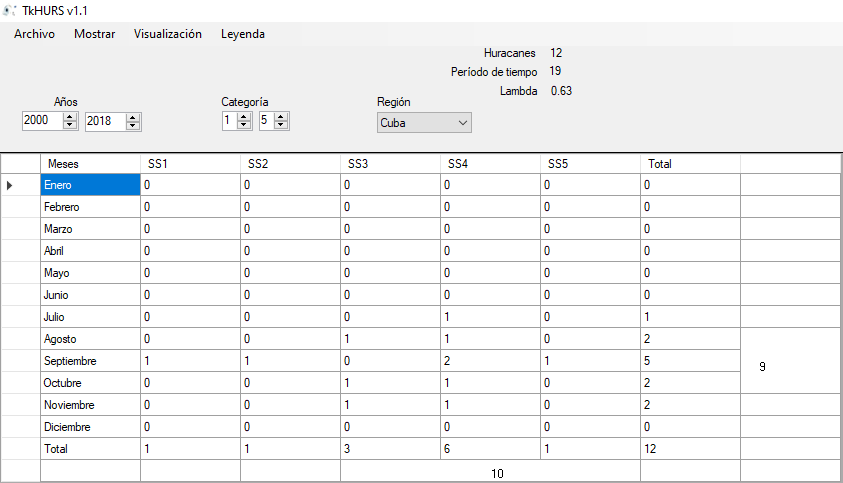
\includegraphics[scale=0.75]{Meses_categoria}
\caption{Meses por categoría}
\label{fig:Meses_categoria}
\end{figure}

\pagebreak

Visualización: muestra las opciones de vista que presenta el software; el “Modo Tabla” es para mostrar todos los datos de interés en dicho formato, “Modo Gráfico” tiene otras 3 opciones propias para elegir el tipo de gráfico en el que se quieran observar los resultados que se presentan en el archivo “.csv” (Gráficos de Barras, Pastel y Línea) y “Modo Mapa” (será implementada en la próxima versión) (Figura \ref{fig:Visualizacion}). %Fue pensado con el objetivo de permitirle al usuario analizar los datos desde distintos puntos de vista (Figura \ref{fig:Visualizacion}).\\

\begin{figure}[H]
\centering
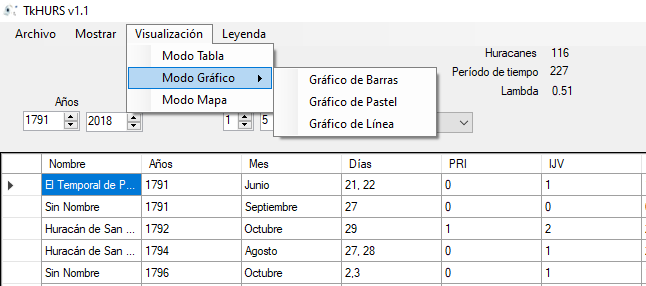
\includegraphics[scale=0.5]{Visualizacion}
\caption{Opciones de visualización}
\label{fig:Visualizacion}
\end{figure}


Gráfico de barras con la opción meses: el gráfico muestra el resultado del filtrado correspondiente luego de haber elegido los meses para el estudio (Figura \ref{fig:grafico_barras}). %Como se aprecia, es posible escoger de cúal en específico se quieren observar los resultados (Figura \ref{fig:grafico_barras}).

\begin{figure}[H]
\centering
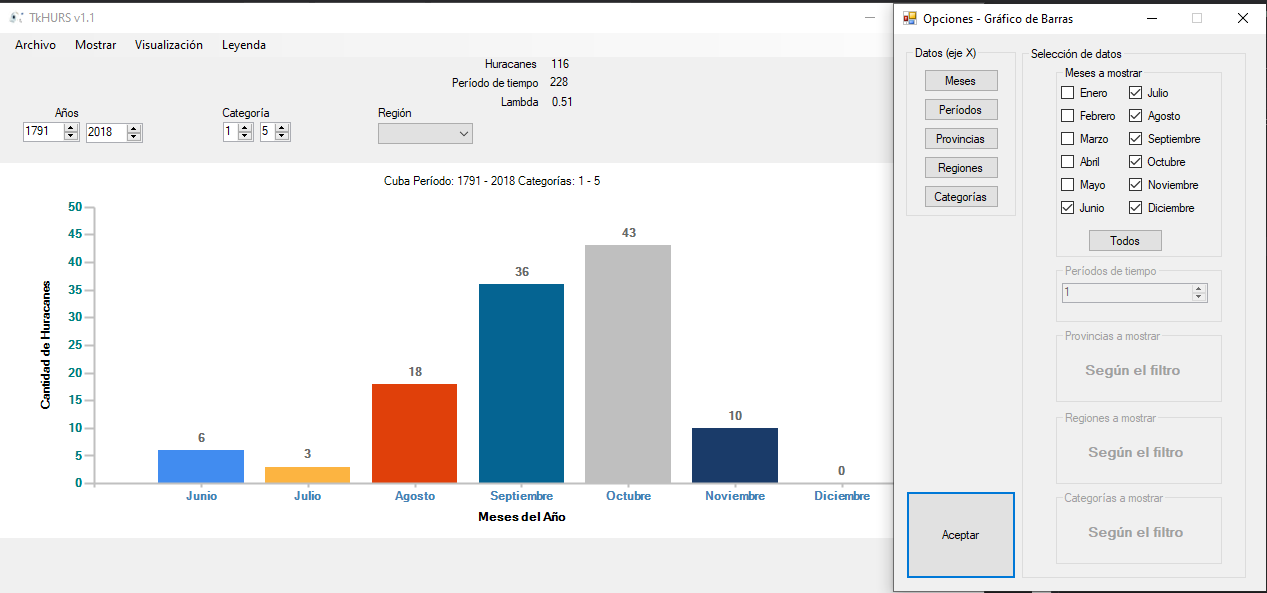
\includegraphics[scale=0.45]{grafico_barras}
\caption{Gráfico de barras (meses por cantidad de huracanes)}
\label{fig:grafico_barras}
\end{figure}

\pagebreak


Gráfico de barras con la opción período: el gráfico muestra el resultado del filtrado correspondiente luego de haber elegido el período de estudio. Como se aprecia, es posible escoger que rango de tiempo desea observar, haciendo sencilla la apreciación y el poder comparar distintos intervalos de tiempo en la historia cubana respecto a huracanes. En el ejemplo de la imagen se escogió un intervalo de 20 años (Figura \ref{fig:grafico_barras_periodo}).

\begin{figure}[H]
\centering
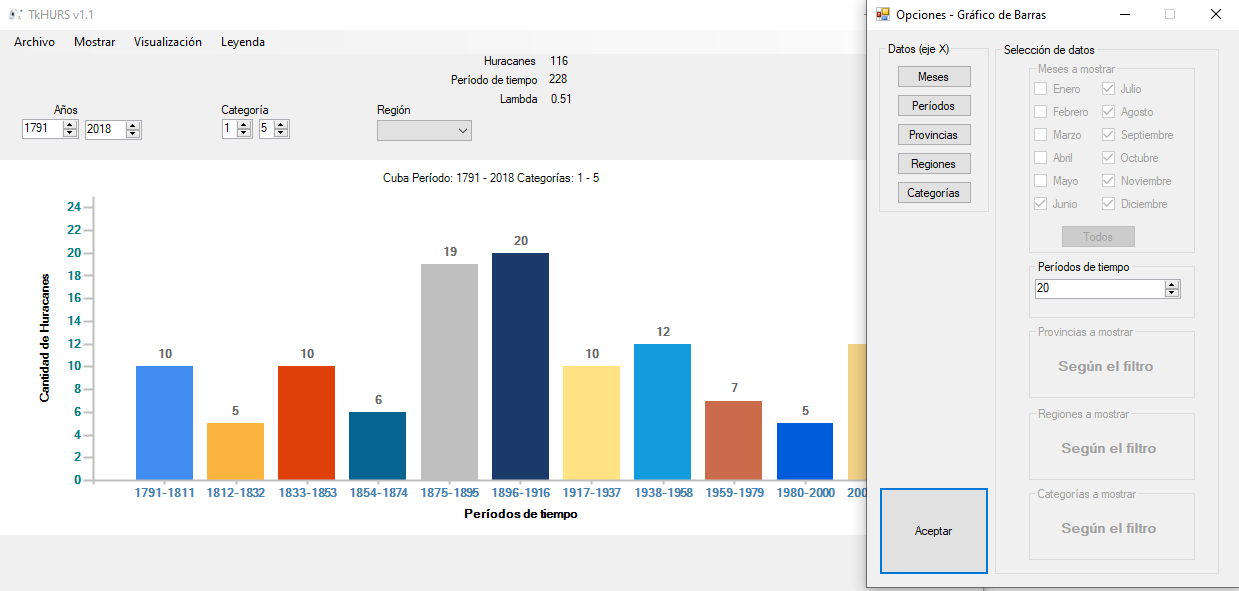
\includegraphics[scale=0.45]{grafico_barras_periodo}
\caption{Gráfico de barras (período de tiempo por cantidad de huracanes)}
\label{fig:grafico_barras_periodo}
\end{figure}

\pagebreak

Gráfico de barras: categorías por cantidad de huracanes, afectado por el filtro como la mayoría de las vistas. Muy útil permitiendo hacer la comparación entre las categorías de huracanes que afectan a Cuba. En la imagen se observa que, teniendo en cuenta la información dada en la cronología, no han llegado a La Isla muchos fenómenos tropicales del máximo valor en la escala de Saffir-Simpson (Figura \ref{fig:grafico_barras_categoria}).

\begin{figure}[H]
\centering
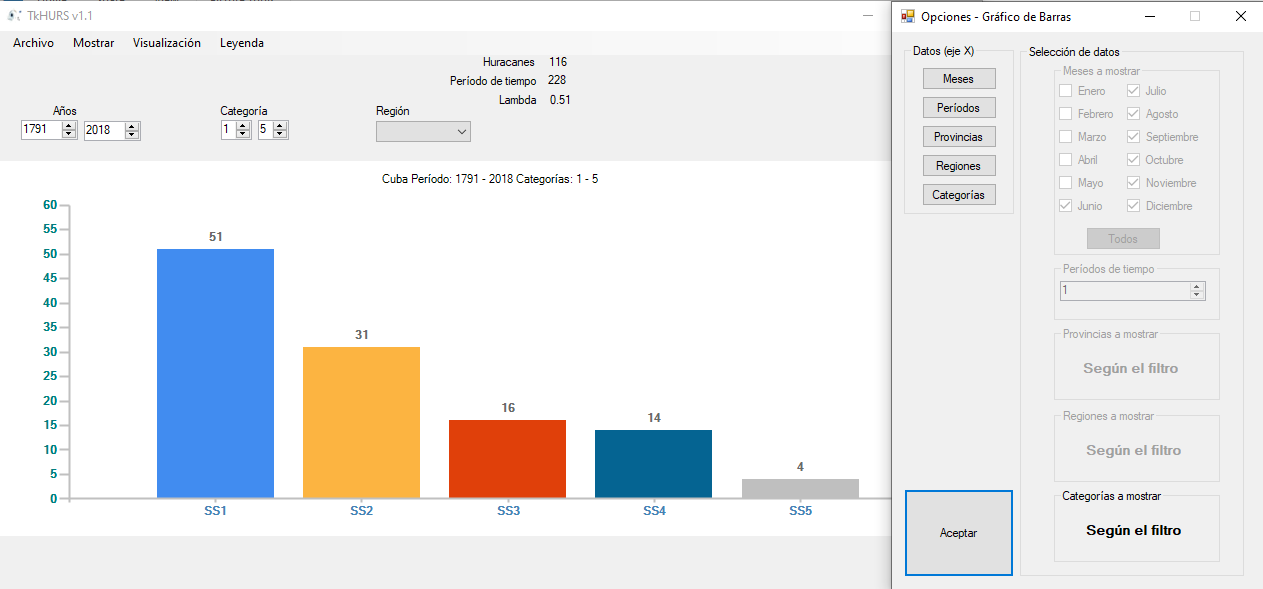
\includegraphics[scale=0.45]{grafico_barras_categoria}
\caption{Gráfico de barras (categorías por cantidad de huracanes)}
\label{fig:grafico_barras_categoria}
\end{figure}

\pagebreak

Gráfico de barras: se muestran las regiones por cantidad de huracanes e igual permite una rápida comparación. Es fácil apreciar cúal ha sido la región más afectada por los huracanes según los registros. Estas observaciones pueden ser de ayuda a la hora de establecer medidas preventivas con el objetivo de evitar pérdidas de vidas humanas y económicas, sabiendo las zonas más afectadas por estos fenómenos atmosféricos (Figura \ref{fig:grafico_barras_regiones}).

\begin{figure}[H]
\centering
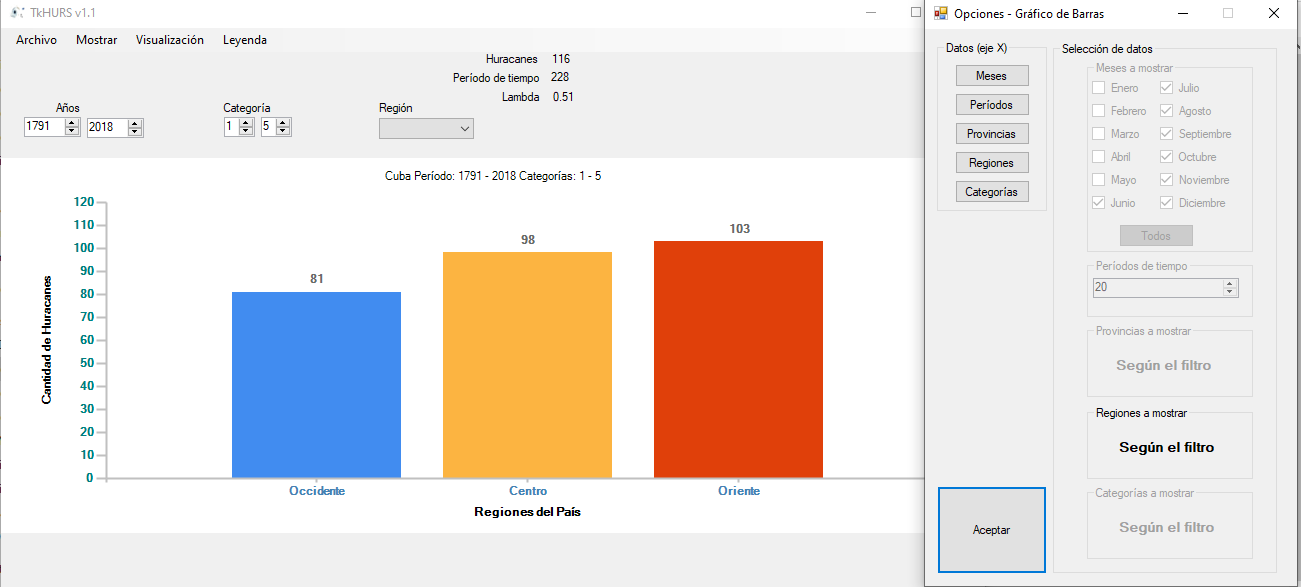
\includegraphics[scale=0.45]{grafico_barras_regiones}
\caption{Gráfico de barras (regiones por cantidad de huracanes)}
\label{fig:grafico_barras_regiones}
\end{figure}

\pagebreak

Gráfico de barras: provincias por cantidad de huracanes. Se aprecian las provincias (y municipio especial) y se puede observar que La Isla de la Juventud ha sido la más azotada por estos eventos meteorológicos a través del tiempo. Dato que no podríamos inferir sólo a partir del gráfico de regiones, por ejemplo (Figura \ref{fig:grafico_barras_provincias}).

\begin{figure}[H]
\centering
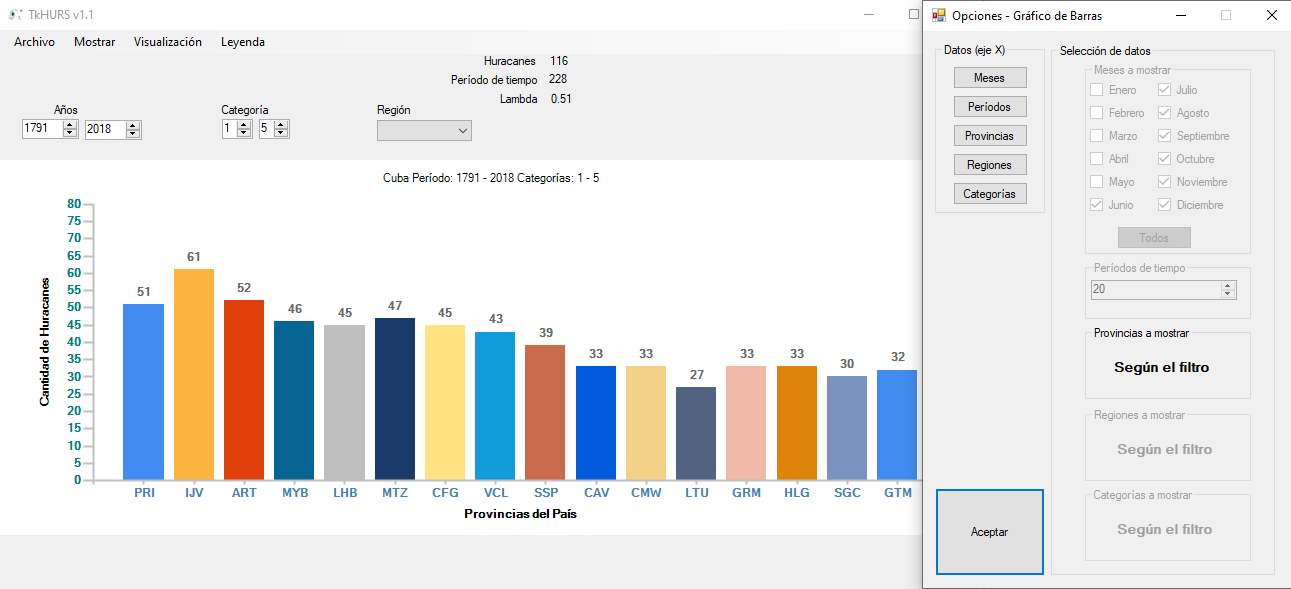
\includegraphics[scale=0.40]{grafico_barras_provincias}
\caption{Gráfico de barras (provincias por cantidad de huracanes)}
\label{fig:grafico_barras_provincias}
\end{figure}



Gráfico de línea: categorías por cantidad de huracanes (Figura \ref{fig:grafico_pastel_prcnt})

\begin{figure}[H]
\centering
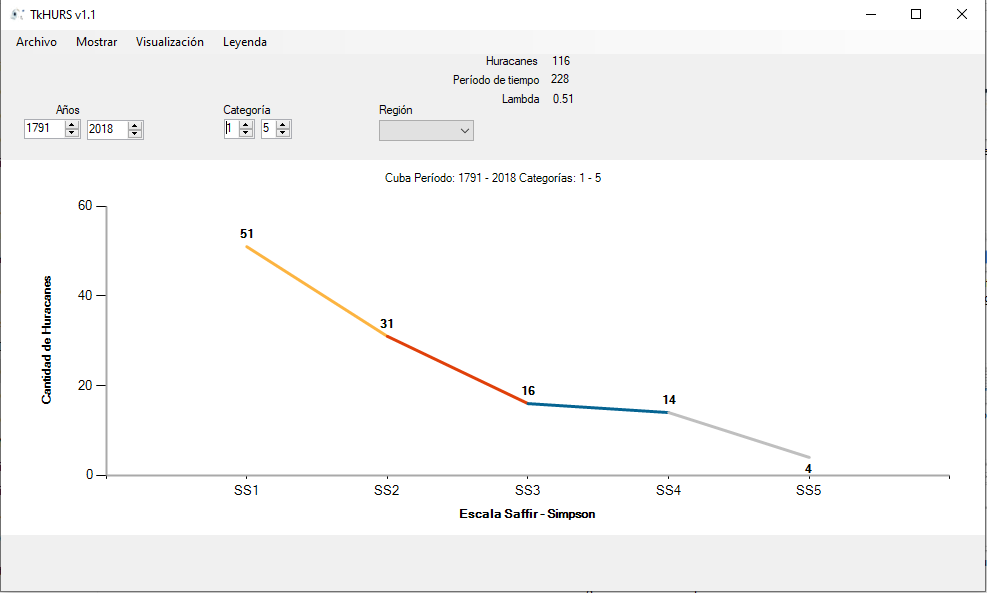
\includegraphics[scale=0.40]{grafico_lineas}
\caption{Gráfico de línea (categorías por cantidad de huracanes)}
\label{fig:grafico_lineas}
\end{figure}

\pagebreak

Gráfico de pastel: categorías por cantidad de huracanes (Figura \ref{fig:grafico_pastel_cant})

\begin{figure}[H]
\centering
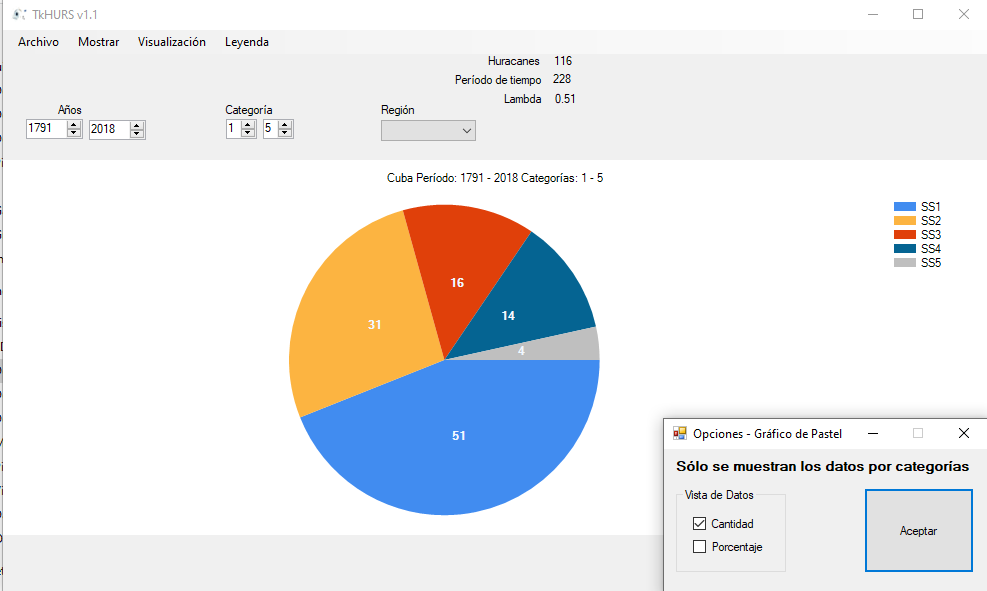
\includegraphics[scale=0.45]{grafico_pastel_cant}
\caption{Gráfico de pastel (categorías por cantidad de huracanes)}
\label{fig:grafico_pastel_cant}
\end{figure}

Gráfico de pastel: categorías por porcentaje de huracanes (Figura \ref{fig:grafico_pastel_prcnt})

\begin{figure}[H]
\centering
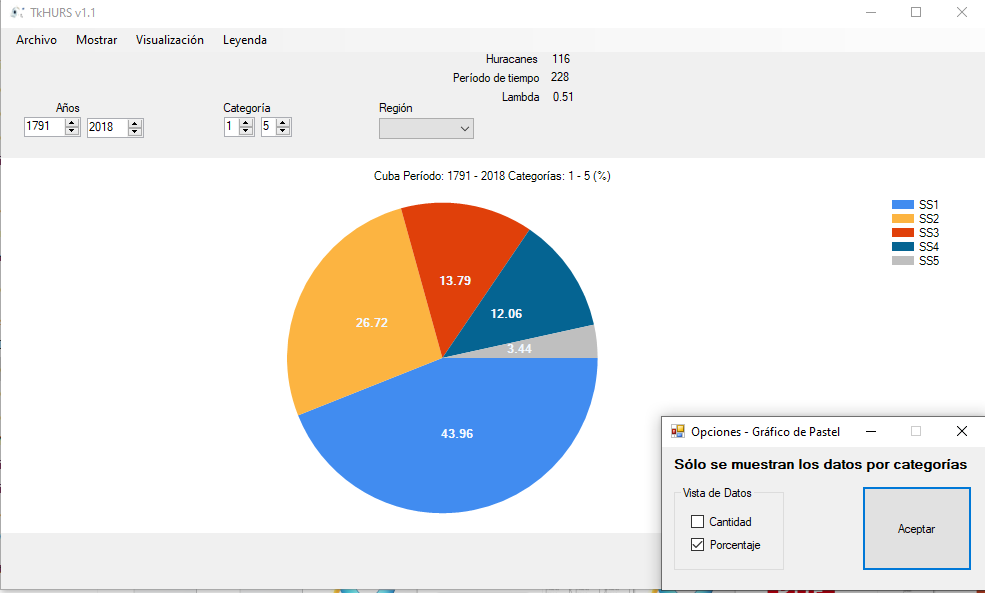
\includegraphics[scale=0.45]{grafico_pastel_prcnt}
\caption{Gráfico de pastel (categorías por porcentaje de huracanes)}
\label{fig:grafico_pastel_prcnt}
\end{figure}

\pagebreak


\subsection{Leyenda}

Esta pestaña se encarga de proporcionar la simbología usada en la aplicación. (Figura \ref{fig:Leyenda}).


\begin{figure}[H]
\centering
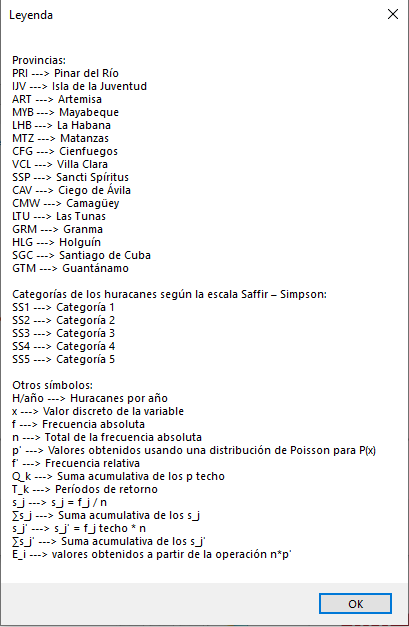
\includegraphics[scale=0.8]{Leyenda}
\caption{Leyenda de la simbología usada }
\label{fig:Leyenda}
\end{figure}

\pagebreak


\subsection{Exportar resultados}

Guardar: se exporta a un Excel toda la información obtenida o se salva una imagen del gráfico que se observe, depende de lo que esté en la pantalla principal. En la figura se observa el resultado de la primera opción (Figura \ref{fig:save}).


\begin{figure}[H]
\centering
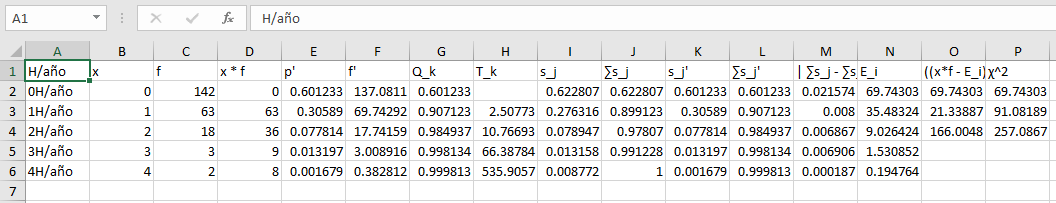
\includegraphics[scale=0.55]{save}
\caption{Datos guardados del análisis de períodos de retorno de huracanes }
\label{fig:save}
\end{figure}


























